\documentclass[12pt]{article}
\usepackage{url,hyperref}
\usepackage{times}
\usepackage[left=1in,right=1in,top=1in,bottom=1in]{geometry}
\usepackage[utf8]{inputenc}
\usepackage{amsmath, xparse}
\usepackage{derivative}
\usepackage[bb=px]{mathalfa}
\usepackage{graphicx}
\usepackage{caption}
\DeclareCaptionFormat{citation}{%
  \ifx\captioncitation\relax\relax\else
    \captioncitation\par
  \fi
  #1#2#3\par}
\newcommand*\setcaptioncitation[1]{\def\captioncitation{\textit{Source:}~#1}}
\let\captioncitation\relax
\captionsetup{format=citation,justification=centering}
\graphicspath{ {./images/} }

\begin{document}

\noindent \textbf{CAP 6640 -- Natural Language Processing\hspace*{\fill}Spring 2025}\\
\noindent{\bf Homework \#2} \hfill Due date: January 31, 2025.

\begin{description}
  \item[Problem 1: ] \hfill %Describe, in your own words, how Artificial Neural Networks (ANN) function and how incorporating multiple layers within an ANN contributes to improved accuracy.
  
  Artificial Neural Networks, or ANNs in short, are a type of computational learning model that are inspired by how the human brain functions. 
  ANNs are composed of computational unit of nodes named as neurons, organized into layers that process the input data and generate an output for tasks such as predictions and classifications.
  First component of the ANN is the input layer, which receives the input data related to the each word vector. Each neuron in this layer represents a feature of the input data.
  The hidden layers, which are located between the input and output layers, contain neurons that apply transformations to relationships by computing a weighted sum of input data 
  and passing the result through an activation function to introduce non-linearity. By incorporating multiple hidden layers, the model can learn complex patterns in the data.
  As a last layer, the output layer generates the final output of the model, which can be used for making predictions or classifications.
  How ANNs do the learning process is by adjusting the weights of the connections between the nodes in the network to minimize the error between the predicted output and the actual output.

  The incorporation of multiple layers within an ANN contributes to improved accuracy by allowing the model to learn complex representations in the data.
  Each hidden layer in the network learns different features of the data, and by stacking multiple layers, the model can learn hierarchical representations of the data.
  Each layer learns increasingly abstract representations. For example, in the context of natural language processing, the first hidden layer might learn simple features such as
  word frequencies, while the second hidden layer might learn more complex features such as word co-occurrences. By learning these hierarchical representations, the model can capture
  complex patterns in the data and make more accurate predictions or classifications.
  Furthermore, adding more layers with non-linear activation functions allows the model to capture highly complex relationships in the data that would be difficult to learn 
  with a simple, and shallow network. In the context of language processing, this can help the model learn the relationships or dependencies between words and phrases.
  Lastly, instead of memorizing the raw data, the model can learn meaningful high-level features to generalize from the data, which can improve its performance on unseen data.
  
  \pagebreak
  
  \item[Problem 2:] \hfill %Provide a mathematical explanation of ANN, including both matrix-based and summation-based representations.

  \begin{enumerate}
    \item \textbf{Summation-based representation}:
    For a single neuron in an Artificial Neural Network (ANN), the output of the neuron can be represented mathematically as:

    \begin{center}
      $\displaystyle{z = \sum_{i=1}^{n} w_i x_i + b}$
    \end{center}

    where $z$ is the weighted sum of the inputs features $x_i$ with corresponding weights $w_i$, $b$ is the bias term, and $n$ is the number of input features 
    used in this neuron calculation.

    The output of the neuron is then passed through an activation function, which introduces non-linearity to the model:

    \begin{center}
      $\displaystyle{a = f(z) = f(\sum_{i=1}^{n} w_i x_i + b)}$
    \end{center}
    
    where $a$ is the final output of the neuron after passing through the activation function $f$.

    If we apply this logic for a single layer with $m$ neurons in an ANN, each neuron computes its output as:

    \begin{center}
      $\displaystyle{z_j = \sum_{i=1}^{n} w_{ji} x_i + b_j}$ for $j = 1, 2, ..., m$
    \end{center}

    where $z_j$ is the weighted sum of the inputs features $x_i$ with corresponding weights $w_{ji}$ and bias term $b_j$ for the $j$-th neuron in the layer.

    The output of the $j$-th neuron is then passed through an activation function:

    \begin{center}
      $\displaystyle{a_j = f(z_j) = f(\sum_{i=1}^{n} w_{ji} x_i + b_j)}$ for $j = 1, 2, ..., m$
    \end{center}

    In summary, the summation-based representation expresses the ANN in terms of individual neurons and connections. 

    \item \textbf{Matrix-based representation}:
    
    The above summation-based representation can be represented in matrix form for a layer of neurons in an ANN. Let's denote the input features as a vector $X$ of size $n$.

    \begin{center}
      $\displaystyle{X = \begin{bmatrix} x_1 \\ x_2 \\ \vdots \\ x_n \end{bmatrix}}$
    \end{center}

    The weights of the connections between the input features and the neurons in the layer can be represented as a weight matrix $W$ of size $m \times n$, where $m$ is the number of neurons in the layer.

    \begin{center}
      $\displaystyle{W = \begin{bmatrix} w_{11} & w_{12} & \cdots & w_{1n} \\ w_{21} & w_{22} & \cdots & w_{2n} \\ \vdots & \vdots & \ddots & \vdots \\ w_{m1} & w_{m2} & \cdots & w_{mn} \end{bmatrix}}$
    \end{center}

    The bias terms for each neuron can be represented as a bias vector $B$ of size $m$.

    \begin{center}
      $\displaystyle{B = \begin{bmatrix} b_1 \\ b_2 \\ \vdots \\ b_m \end{bmatrix}}$
    \end{center}

    By combining all these, the weighted sum of the inputs for all neurons in the layer can be computed as a matrix multiplication as

    \begin{center}
      $\displaystyle{Z = W \cdot X + B}$
    \end{center}

    As the last step, by applying the activation function element-wise to the matrix $Z$, we can compute the output of all activated neurons in the layer as

    \begin{center}
      $\displaystyle{A = f(Z) = f([z_1, z_2, \cdots , z_n]) = [f(z_1), f(z_2), \cdots , f(z_n)]}$
    \end{center}

    where $A$ is the output of the layer after passing through the activation function $f$. 

    In summary, this matrix-based representation makes computations more efficient by leveraging vectorized operations.

  \end{enumerate}

  \pagebreak

  \item[Problem 3:] \hfill %Discuss the challenges associated with named entities and explain how window classification addresses these challenges.
  
  Named Entity Recognition, or NER in short, is the task of identifying and classifying named entities in text into predefined categories such as person names, 
  organization names, locations, etc.
  However, NER faces several challenges that makes it a difficult task. Some of the challenges associated with named entities are:

  \begin{enumerate}
    \item \textbf{Ambiguity in Entities}: Named entities can be ambiguous, meaning that the same word can refer to different entities based on the context. 
    For example, the word "Acibadem" in Turkish can refer to a dessert, a neighbourhood in Istanbul, or the healthcare group organization.

    \item \textbf{Handling Unknown or Emerging Entities}: NER systems need to be able to handle unknown or emerging entities that are not present in the training data.
    For instance, probably a system trained on before 2020 data would not recognize the entity "COVID-19" as a disease and classify it as unknown word or a generic word. 

    \item \textbf{Ambiguity}: Named entities can be ambiguous, meaning that it is not obvious to predict whether it is an entity or just a general term used in the text.
    To give an example, Open AI, can be considered as an entity, but "open" and "AI" can be considered as separate words and can be interpreted as open-source AI.
    
    \item \textbf{Complex Named Entities and the Boundries}: Named entities can be complex and composed of multiple words which makes it difficult to identify the boundaries of the entity.
    To give an instance, "Washington Post Sanctions" can be considered as a news organization entity, but also can be composed of multiple components such as administration in Washington D.C., etc.
  \end{enumerate}

  To address these challenges, window classification technique can be used in NER. Window classification involves dividing the text into fixed-size windows
  to capture the context around each word. By considering the context around each word, the model can better understand the meaning of the word and disambiguate named entities.

  To illustrate, consider the sentence "Jordan Thompson traveled to Jordan.". In this sentence, the word "Jordan" appears twice, but has different meanings.
  By using a window classification approach, the model can consider the context around each occurrence of "Jordan" to determine whether it refers to a person's name or a location.
  However, we might fail to capture the positional information and contextual nuances of the entities in the text if we use a very simple averaging method for the word vectors in the context window.
  To address this issue, we can use more sophisticated methods such as softmax classifier to calculate the probability of each word in the context window to be the entity of interest appearing together.
  By using window classification, the model can better handle ambiguity, unknown entities, and complex named entities by considering the context around each word.

  \pagebreak

  \item[Problem 4:] \hfill %Describe the backpropagation algorithm, both conceptually in your own words and mathematically.
  
  Backpropagation is an algorithm used in ANNs to adjust the weights of the connections between neurons in the network to minimize the error between the predicted output 
  and the actual output.
  An input from the input layer is fed forward through the network, and the output is compared to the actual output to calculate the error. This mechnism is called forward pass.
  The error is then propagated backward through the network to adjust the weights of the connections, which is called backpropagation. Mathematically, partial derivatives of the loss
  with respect to the weights are calculated using the chain rule of calculus, and the weights are updated in the opposite direction of the gradient to minimize the loss in future predictions.
  We repeat this process iteratively until the model converges to a set of optimal weights that minimize the error.

  To explain the backpropagation algorithm visually, we will consider the following operations on our NN:

  \begin{figure}[h]
    \centering
    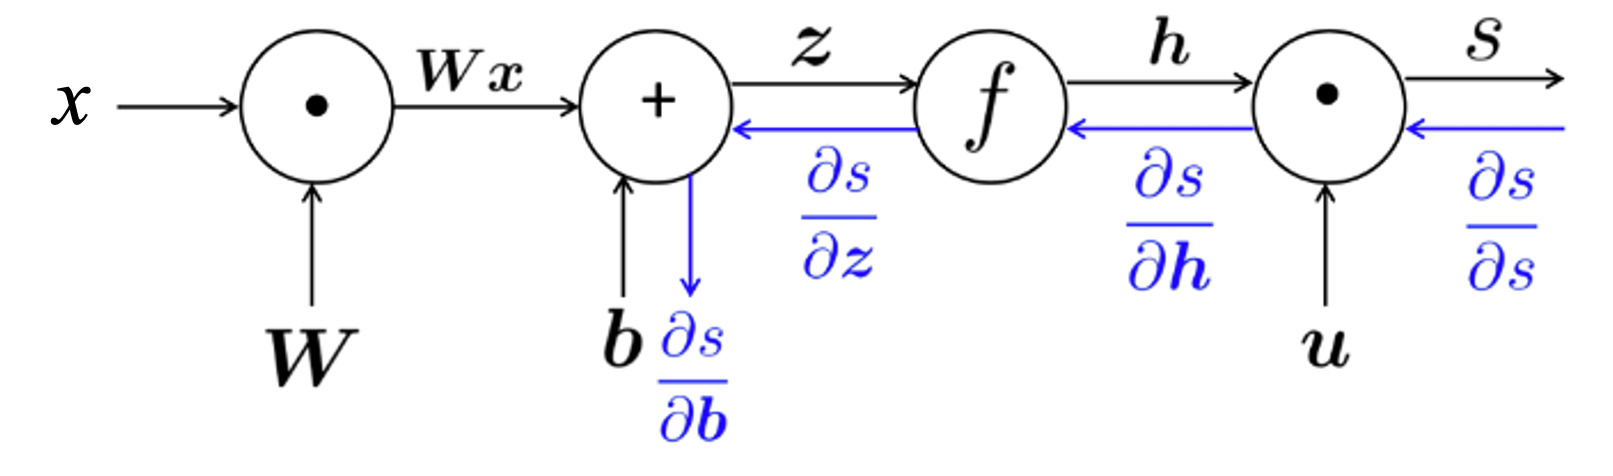
\includegraphics[width=0.8\textwidth]{Picture1.png}
    \setcaptioncitation{Source: Mohaisen, D. (2025). Lecture 6: Pitfalls in Word Vectors and Backpropagation
    [PowerPoint slides]. University of Central Florida Computer Understanding of Natural Language: http://www.cs.ucf.edu/}
    \caption{Example of a basic Neural Network operations for backpropagation}
  \end{figure}

  In our single node network, we have an input $x$, a weight $w$, a bias $b$, an activation function $f$, and $u$ to normalize the activated neuron to a score. First, we calculate the
  weighted sum of the input and the weight, and add the bias term to get the preactived value $z$ as 

  \begin{center}
    $z = Wx + b$
  \end{center}

  Then, we pass the $z$ value to an activation function $f$ to introduce non-linearity to the model and get the activated value $h$ as

  \begin{center}
    $h = f(z)$
  \end{center}

  Finally, we normalize the activated value $h$ to a score $s$ as

  \begin{center}
    $s = u^Th$
  \end{center}

  Our goal is to minimize the error between the predicted score $s$ and the actual score $y$. To achieve this, we calculate the loss function $L$, assuming that we use the mean squared difference between
  the predicted score and the actual score as the loss function. Then the loss function is calculated as

  \begin{center}
    $\displaystyle{L = loss(\hat{y}, y) = \frac{1}{2}(y - s)^2}$
  \end{center}

  To minimize the loss function, we need to calculate the gradient of the loss function with respect to the model parameters, which are weights $W$, the bias $b$, and $u$.
  Backpropagation follows the chain rule, which helps compute derivatives layer by layer as seen from the Figure 1.

  The first step is to calculate the gradient of the loss function with respect to the score $s$ as

  \begin{center}
    $\displaystyle{\pdv{L}{s} = (s - y)}$
  \end{center}

  To update the model parameter $u$, using the chain rule, we calculate the gradient of the loss function with respect to the score $s$ as

  \begin{center}
    $\displaystyle{\pdv{s}{u} =  h}$ since $s = u^Th$

    $\displaystyle{\pdv{L}{u} = \pdv{L}{s} \cdot \pdv{s}{u} = (s - y) \cdot h}$
  \end{center}

  Then, the computed gradient is used in gradient descent to update weight $u$ as

  \begin{center}
    $\displaystyle{u^{new} = u^{old} - \eta \pdv{L}{u}}$
  \end{center}

  where $\eta$ is the learning rate that controls the size of the weight updates. The same process is repeated for the weights $W$ and the bias $b$ to minimize the loss function.

  Then, we calculate the gradient of the loss function with respect to the activated value $h$ by assigning the downstream as the upstream gradient times the local gradient as

  \begin{center}
    $\displaystyle{\pdv{s}{h} =  u}$ since $s = u^Th$

    $\displaystyle{\pdv{L}{h} = \pdv{L}{s} \cdot \pdv{s}{h} = (s - y) \cdot u}$
  \end{center}

  Next, we backpropagate the gradient to the preactivated value $z$ by calculating the gradient of the loss function with respect to the preactivated value $z$ as

  \begin{center}
    $\displaystyle{\pdv{h}{z} = f'(z)}$

    $\displaystyle{\pdv{L}{z} = \pdv{L}{h} \cdot \pdv{h}{z} = (s - y) \cdot u \cdot f'(z)}$
  \end{center}

  Finally, as the last backpropagation, we calculate the gradient of the loss function with respect to the weights $W$ and the bias $b$ as

  \begin{center}
    $\displaystyle{\pdv{z}{W} = x}$ since $z = Wx + b$

    $\displaystyle{\pdv{L}{W} = \pdv{L}{z} \cdot \pdv{z}{W} = (s - y) \cdot u \cdot f'(z) \cdot x}$

    $\displaystyle{\pdv{z}{b} = 1}$ since $z = Wx + b$

    $\displaystyle{\pdv{L}{b} = \pdv{L}{z} \cdot \pdv{z}{b} = (s - y) \cdot u \cdot f'(z) \cdot 1}$
  \end{center}

  Using those gradients, we can update the weights $W$ and the bias $b$ to minimize the loss function as follows:

  \begin{center}
    $\displaystyle{W^{new} = W^{old} - \eta \pdv{L}{W}}$

    $\displaystyle{b^{new} = b^{old} - \eta \pdv{L}{b}}$
  \end{center}

  The key takeaway from the backpropagation algorithm is that it allows the model to learn the optimal weights that minimize the error between the predicted output and the actual output.
  Mathematically, we need to go through the chain rule to calculate the gradients of the loss function with respect to the model parameters and update the weights in the opposite direction of the gradient.
  Depending on the size of the model parameters, the backpropagation algorithm can be computationally expensive, but it is a powerful algorithm that enables the model to learn complex patterns in the data.

  \pagebreak

  \item[Problem 5:] \hfill %Explain the necessity of structures for analyzing language dependencies.
  
  In NLP, understanding language dependencies and sentence structures, which is uncovering the relationships between words in a sentence, is crucial for accurately interpreting
  meaning. To achieve this, dependency parsing and structure analysis are used to identify the relationships between words in a sentence and represent them in a structured format.
  They especially help in understanding the syntactic and semantic relationships between words, as without them the meaning of the sentence can be ambiguous or unclear. For 
  instance, in the sentence "The girl painted the picture with the brush.", the ambiguity arises because "with the brush" can modify either "painted", explaining how she painted,
  or "the picture", describing the content of the picture.

  The necessity of structures for analyzing language dependencies can be summarized as follows:

  \begin{enumerate}
    \item \textbf{Resolving Ambiguity}: Structures help disambiguate the meaning of words in a sentence by identifying the relationships between words. For example, in the example
    sentence above, dependency parsing can help determine whether "with the brush" modifies "painted" or "the picture". This is crucial for accurate understanding of the sentence.
    Dependency structures and similar structures help disambiguate relationships by showing how words are connected.

    \item \textbf{Representing Hierarchical Relationships}: Sentences mostly have main clauses and modifiers, requiring hierarchical understanding. Uncovering these relationships
    helps to decode the important points and thw flow of the sentence. For example, in the sentence "the tall building with glass windows.", "tall" modifies "building," while "glass" 
    modifies "windows". Dependency structures, especially tree or graph like structrues, can represent these hierarchical relationships.

    \item \textbf{Precision and Meaningful Communication}: Every human language tends to allow complex sentences and structures, mostly by combining multiple clauses and phrases
    into larger textual components. These longer sentences captures more precision by adding details and nuances, and also helps to define the relationships between the object and subject.
    
  \end{enumerate}

  \pagebreak

  \item[Problem 6:] \hfill %Describe the stochastic gradient descent algorithm, how it works, and the types of problems it aims to address within the context of the gradient descent algorithm.
  
  Gradient descent (GD) algorithm is a basic optimization algorithm used to minimize the loss or cost function $J(\theta)$ of a model by adjusting the weights of the connections between neurons in the ANN.
  It works by iteratively updating the weights in the opposite direction of the gradient of the loss function with respect to the weights. The update rule for the weights matrix is given by:

  \begin{center}
    $\displaystyle{\theta^{new} = \theta^{old} - \eta \nabla_{\theta} J(\theta)}$
  \end{center}
  
  where $\theta$ represents the weights of the model, $\eta$ is the learning rate that controls the size of the weight updates, and $\nabla J(\theta)$ is the gradient of the 
  loss function with respect to the weights.

  However, in the context of NLP, the training data can be very large, and computing the gradient over the entire corpus can be computationally expensive. Furthermore, 
  in the case of large datasets, the waiting time to update the weights can be very long. To address these issues, stochastic gradient descent (SGD) algorithm is used.

  SGD is a variant of the GD algorithm that updates the weights based on a single training example windows or a mini-batch of examples, rather than the entire dataset. This makes it 
  much faster and well-suited for large-scale problems. The update rule for the weights using SGD is given by:

  \begin{center}
    $\displaystyle{\theta^{new} = \theta^{old} - \eta \nabla_{\theta} J(\theta; x_i, y_i)}$
  \end{center}

  where $(x_i, y_i)$ is a training example, and $\nabla_{\theta} J(\theta; x_i, y_i)$ is the gradient of the loss function with respect to the weights for the training example.
  The weights are updated for each training example or mini-batch of examples, which speeds up the training process and makes it more efficient. So the main advantage of SGD 
  is that it is computationally efficient and can handle large datasets.

  Like in GD, in SGD, we select random samples and update model parameters until the model converges to a stopping condition such as local minimum or small gradient updates.

  \pagebreak

  \item[Problem 7:] \hfill %Explain the skip-gram model with negative sampling and how it operates.
  
  Skip-gram model is a type of word embedding model that learns distributed representations of word embeddings in a continuous vector space based on their spatial proximity 
  to other words. The skip-gram model tries to predict the surrounding context words $w_{context}$ given a target word $w_{target}$, by maximizing the probability of observing
  the context words given the target word based on their co-occurrences in the corpus. 

  For example, in the sentence "Apple released iOS 18.3 for iPhone", assuming that the target word is "iOS", the skip-gram mode tries to predict nearby context words like 
  "Apple", "released", and "iPhone".

  In general, we calculate the probability of observing the context words given the target word as

  \begin{center}
    $\displaystyle{P(w_{context} | w_{target}) = \frac{\exp({u_{w_{context}}^T v_{w_{target}}})}{\sum_{w \in V} \exp({u_{w}^T v_{w_{target}}})}}$
  \end{center}

  where $u_{w_{context}}$ and $v_{w_{target}}$ are the word embeddings or vectors for the context word and target word, respectively, and $V$ is the vocabulary of words in the corpus.

  However, the pitfall of the skip-gram model is the normalization done at the denominator over the entire vocabulary, which can be computationally expensive and a slow process 
  for a large corpus. To address this issue, we make the skip-gram efficient by introducing skip-gram model with negative sampling.

  The skip-gram model with negative sampling is an extension of the skip-gram model that addresses the computational inefficiency of the original model. Instead of calculating
  the probability of observing the context words given the target word over the entire vocabulary, negative sampling only updates a few words per training step instead of the 
  entire vocabulary and approximates the probability by sampling a small number of negative words or random noise, namely the words that are not in the context, and comparing 
  them to the true context words. For a given target word $w_{target}$, the model is trained to maximize the probability of observing the true context words, and futhermore 
  minimize the probability of observing the sampled $k$ negative words, which are the random words that do not appear in the context.

  The new and additional objective function for the skip-gram model with negative sampling is

  \begin{center}
    $\displaystyle{L(\theta) = \log \sigma(u_{w_{context}}^T v_{w_{target}}) + \sum_{i=1}^{k}{\mathbb{E}_{w_i \sim P(w)} [\log \sigma(-u_{w_{i}}^T v_{w_{target}})]}}$
  \end{center}

  where $\sigma$ is the sigmoid function, $u_{w_{context}}$ and $v_{w_{target}}$ are the word embeddings for the context word and target word, respectively, $P(w)$ is a noise 
  distribution, and $k$ is the number of negative samples.

  With the introduction of negative sampling, the skip-gram model becomes more computationally efficient since instead of summing over millions of words, 
  we sum over just a few negative samples. In addition, the model can learn more accurate word embeddings as the model learns better vector representations by pushing correct 
  pairs closer while separating unrelated words.

  \pagebreak

  \item[Problem 8:] \hfill %Discuss the two approaches for evaluating word embeddings (vectors), namely intrinsic and extrinsic evaluations, along with their respective advantages and disadvantages.
  
  Dense word representations, or word embeddings, are vector representations of words in a continuous vector space that capture the semantic and syntactic relationships between 
  words.
  Evaluating the quality of word embeddings is crucial to ensure that the embeddings capture meaningful relationships between words and can be used effectively in NLP tasks.

  There are two main approaches for evaluating word embeddings:

  \begin{enumerate}
    \item \textbf{Intrinsic Evaluation}: Intrinsic evaluation involves evaluating the quality of word embeddings based on their performance on specific linguistic tasks such as
    
    \begin{itemize}
      \item Qualitative analysis, which involves visually inspecting the word embeddings to understand the relationships between words.
      \item Clustering, which groups similar words together based on their word embeddings and evaluates the quality of the clusters.
      \item Word analogy, which evaluates the ability of word embeddings to capture semantic relationships between words by solving analogy tasks on large word analogy datasets.
      \item Word similarity, which measures the similarity between word embeddings based on their cosine similarity or Euclidean distance, and compares it to human judgments of word similarity.
    \end{itemize}

    Advantages of intrinsic evaluation include:

    \begin{itemize}
      \item Direct evaluation of the quality of word embeddings regardless of the NLP task.
      \item Does not require training a model on a downstream task, hence it is fast and computationally cheap to perform.
    \end{itemize}

    Disadvantages of intrinsic evaluation include:

    \begin{itemize}
      \item Limited scope of evaluation, as it only evaluates the quality of word embeddings on specific linguistic tasks. Hence, may not reflect the performance of word 
      embeddings on real-world NLP tasks.
    \end{itemize}

  \item \textbf{Extrinsic Evaluation}: Extrinsic evaluation involves evaluating the quality of word embeddings based on their performance on downstream NLP tasks such as
  
  \begin{itemize}
    \item Question answering, which evaluates the ability of word embeddings to answer questions correctly based on a given context.
    \item Machine translation, which evaluates the quality of word embeddings in translating valid text from one language to another.
    \item Named entity recognition (NER), which evaluates the ability of word embeddings to identify named entities in text.
    \item Text classification, which evaluates the quality of word embeddings as inputs in classifying text into predefined categories.
  \end{itemize}

  Advantages of extrinsic evaluation include:

  \begin{itemize}
    \item Evaluates the quality of word embeddings based on their performance on real-world NLP tasks, providing a more practical assessment of the embeddings.
    \item Evaluates the ability of word embeddings to generalize to unseen data and tasks.
  \end{itemize}

  Disadvantages of extrinsic evaluation include:

  \begin{itemize}
    \item Requires training a model on a real-NLP task, which can be computationally expensive and time-consuming.
    \item Performance on a downstream task may be influenced by factors other than the quality of word embeddings, such as the architecture of the model or the size of the training data.
    \item Slower to test different word embeddings since it requires retraining the model on each new set of embeddings.
  \end{itemize}

  \end{enumerate}

  \pagebreak

  \item[Problem 9:] \hfill %Define word sense, its purpose, and how it is used in practical applications.
  
  Word sense refers to the different meanings or interpretations of a word based on the context in which it appears. Words can have multiple senses or meanings, and the correct
  interpretation of a word depends on the context in which it is used. To give an instance, the word "runner" can refer to a person who runs as an athlete like in the sentence 
  "Sonic was a fast runner.", or a person who smuggles goods like in the sentence "The drug runner was arrested at the border.". We treat each of these distinct meanings as a 
  separate word sense.

  There are several cases in which word sense helps in NLP tasks. As seen from the above, distinguishing between different meanings of a word in a given context helps us to 
  disambiguate the meaning of the word and improve the performance of NLP tasks, since this a common case in every language. This helps for an improved NLP understanding which in
  turn helps for more refined information retrieval.

  To achieve this, it is important to use different contextual word embeddings for each word sense to capture the distinct meanings of the word based on the context, unlike the static 
  vector approach from Word2Vec technique which might result distorted. Nowadays, models like BERT can eliminate these ambiguities on the shot.

  In practical applications, word sense is used in various practical NLP applications such as:

  \begin{enumerate}
    \item \textbf{Machine Translation}: In machine translation, word sense ensures to translate words accurately based on their context and meaning.
    
    \begin{itemize}
      \item "Ne güzel güldün." in Turkish can be translated as "You laughed so beautifully." or "You smiled so beautifully." based on the context.
      \item "Ne güzel bir güldü." in Turkish can be translated as "What a beautiful rose." based on the context.
    \end{itemize}
    
    \item \textbf{Information Retrieval}: In information retrieval, word sense improves the accuracy of search results.
  
    \begin{itemize}
      \item Searching for "apple" can return results related to the fruit or the technology company based on the context.
    \end{itemize}
    
    \item \textbf{Question Answering}: In question answering, word sense helps to understand the meaning of the question and provide accurate answers.
    
    \begin{itemize}
      \item A medical chatbot must differentiate between "nerve" (the optic fiber for transmitting pulses) vs. "nerve" (mental calmness).
    \end{itemize}
    
    \item \textbf{Sentiment Analysis}: In sentiment analysis, word sense helps to identify the sentiment of a word based on its context and meaning.
    
    \begin{itemize}
      \item "The sudden bang scared everyone in the room.", where "bang" refers to a loud noise, which is a negative (fear, surprise) sentiment.
      \item "The party started with a bang.", where "bang" refers to an excitement or success, which is a positive (enthusiasm) sentiment.
    \end{itemize}

  \end{enumerate}

  Closely related with word sense, global context, which refers to the broader textual information that helps determine the meaning of a word, is also important such that
  if the immediate context is unclear, the overall topic or document meaning can guide sense selection. This is actually the main idea behind the BERT model, which improves
  the coherence both in NLP models and tasks.

  \pagebreak

  \item[Problem 10:] \hfill %Explain the max-margin loss function in the context of binary classification for Named Entity Recognition (NER) location identification.
  
  Named Entity Recognition (NER) involves classifying words into entity types, in which one of those types is LOCATION (LOC). In a binary classification setup for 
  location identification, we try to assign a binary label to each word in the text, indicating whether it is a location or not. To be able to classify the words as location
  or not, we try to learn a neural activation function to compute the window's score and based on this score, we do the classification. However, the model can make mistakes
  in the classification, and the max-margin loss function is used to penalize these corrupted windows scoress $S_c$ and encourage the model to calculate higher scores for the 
  true windows $S$. The max-margin loss ensures that correct classifications $S$ have a margin of at least 1 from the decision boundary $S_c$. The loss function can be defined as:

  \begin{center}
    $\displaystyle{L = \max(0, 1 - S + S_c)}$
  \end{center}
  
  where $N$ is the number of windows in the training data, $S$ is the score of the true window, and $S_c$ is the score of the corrupted window. To minimize the loss, the model
  needs to update the weights to increase the score of the true window and decrease the score of the corrupted window. Optimization of the model requires gradient of the loss 
  function with respect to the weights and update the weights using the backpropagation algorithm. Instead of computing gradients over the entire dataset, we can use stochastic
  gradient descent to update the weights based on a single training example or a mini-batch of examples. For each training step with a sample $(x_i, y_i)$, we update the weights
  as

  \begin{center}
    $\displaystyle{W = W - \eta \pdv{L}{W}}$
  \end{center}

  where $\eta$ is the learning rate. Thus, for each training word, we only update the weights if the loss is greater than 0, which encourages the model to learn the correct 
  classification. This approach can speed up the training process and make the model more efficient in learning the correct classification of the windows. 

  \pagebreak
  
\end{description}

\end{document}